\documentclass[12pt]{beamer}

\usepackage[ruled,linesnumbered,titlenotnumbered]{algorithm2e}
\usepackage{color}
\usepackage{hyperref}

\newcommand*{\email}[1]{\href{mailto:#1}{\nolinkurl{#1}} }

\usetheme{Antibes}

\title{Big Data Analytics: London Crime Data Analysis}
\author{Gianmarco Ricciarelli\inst{1}}
\institute{\inst{1}University of Pisa, \\
           \email{gianmarcoricciarelli@gmail.com}}

\date{}

\graphicspath{{../imgs/}}

\setlength\parindent{0pt}

\begin{document}
    \maketitle

    \begin{frame}{Overview}
        \tableofcontents
    \end{frame}

    \section{Introduction} % (fold)
    \label{sec:introduction}
        \begin{frame}{The analysis' purpose}
            To discover the patterns among the criminal activities in the London metropolitan area in a
            distinct window of time.
        \end{frame}

        \begin{frame}{The Dataset(1)}
            \href{https://www.kaggle.com/jboysen/london-crime}{\textbf{London Crime Data, 2008-2016}}: this
            dataset, hosted by \href{https://www.kaggle.com}{\textbf{Kaggle}}, is composed by $13$
            millions rows describing the London metropolitan area's criminal activities by \textit{Borough},
            \textit{Category}, \textit{Month} and \textit{Year} in a window of time that ranges from
            January $2008$ to December $2016$.
        \end{frame}

        \begin{frame}{The Dataset(2)}
            The dataset is composed by $7$ variables:

            \begin{itemize}
                \item \textbf{lsoa\_code}: code for Lower Super Output Area in Greater London;
                \item \textbf{borough}: common name for London borough;
                \item \textbf{major\_category}: high level categorization of crime;
                \item \textbf{minor\_category}: low level categorization of crime within major category;
                \item \textbf{year}: year of reported counts, $2008-2016$;
                \item \textbf{month}: month of reported counts, $1-12$;
                \item \textbf{value}: monthly reported count of categorical crime in given borough;
            \end{itemize}
        \end{frame}

        \begin{frame}{The Dataset(3)}
            The variables \textit{lsoa\_code}, \textit{borough}, \textit{major\_category},
            \textit{minor\_category}, \textit{year} and \textit{month} are \textbf{categorical} variables,
            while \textit{value} is a \textbf{discrete numerical} variable.
        \end{frame}
    % section introduction (end)

    \section{Data Understanding} % (fold)
    \label{sec:data_understanding}
        \begin{frame}{Numeric Variables' Analysis(1)}
            \textbf{value} is the only numeric variables in the dataset, it represents the monthly reported
            count of categorical crime in given borough and has 247 unique values. Its minimum value is 0 and
            its maximum value is 309, the mode is 0, which appears in the 74.56\% of the dataset's samples.
        \end{frame}

        \begin{frame}{Numeric Variables' Analysis(2)}
            Since 10,071,505, that is, the 74.56\% of the dataset's samples have the variable value eguals to
            0, we can conclude that, on a superficial level, the window of time from 2008 to 2016 wasn't too
            dense of criminal activities.
        \end{frame}

        \begin{frame}{Crimes per Year}
            \begin{figure}
                \centering
                \resizebox{\textwidth}{!}{
                    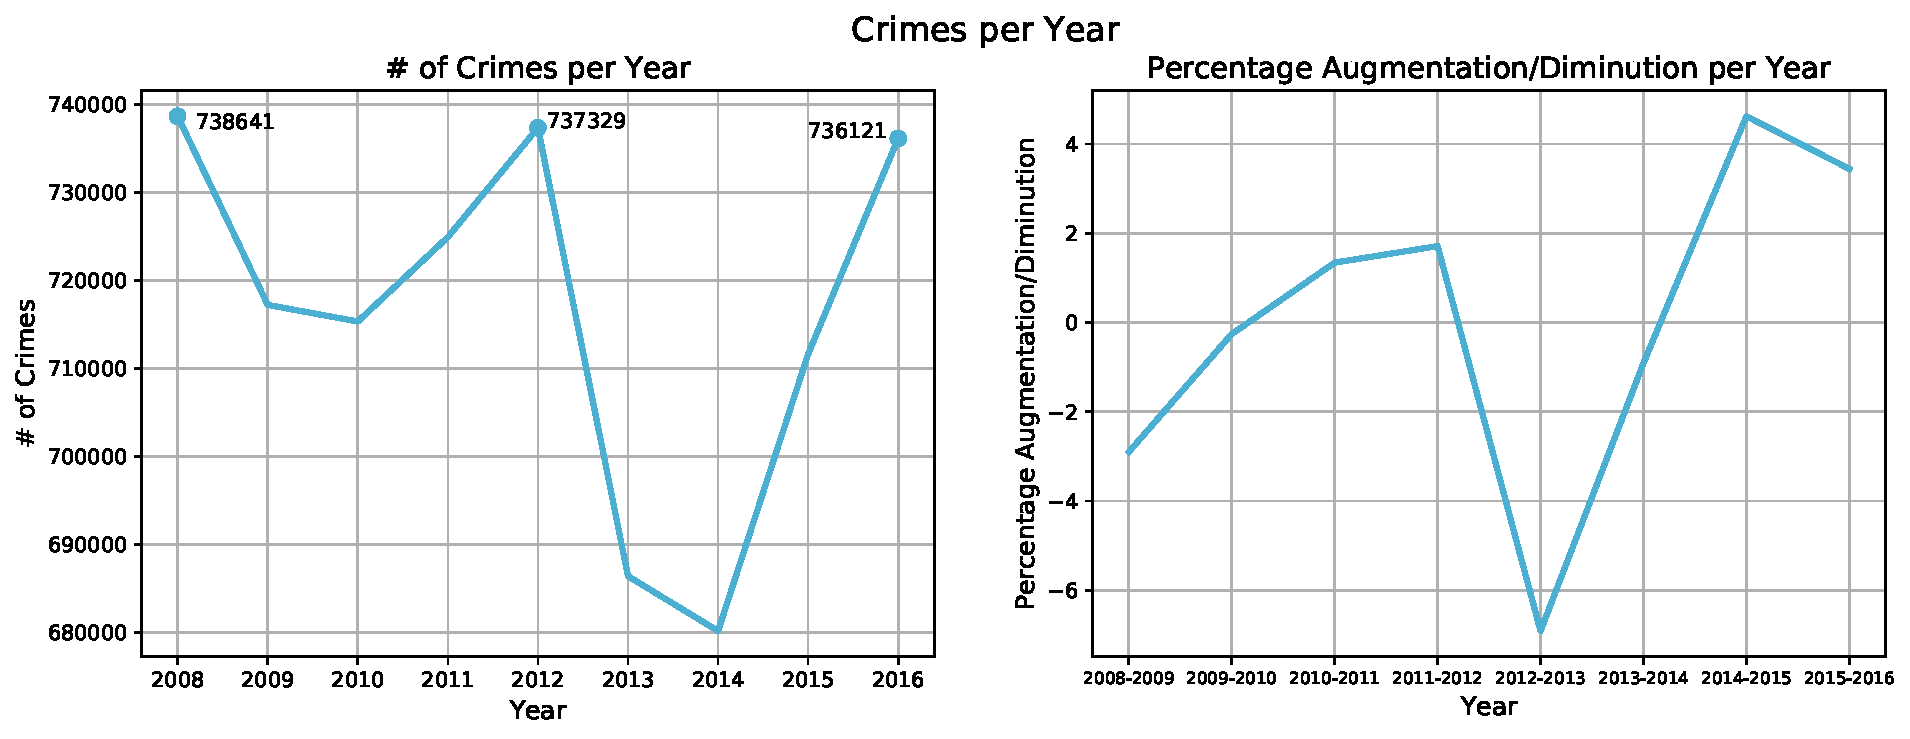
\includegraphics{../imgs/data_understanding/crimes_per_year.pdf}
                }
                \caption{Crime's progress over the years}
            \end{figure}
        \end{frame}

        \begin{frame}{Crimes per Month}
            \begin{figure}
                \centering
                \resizebox{\textwidth}{!}{
                    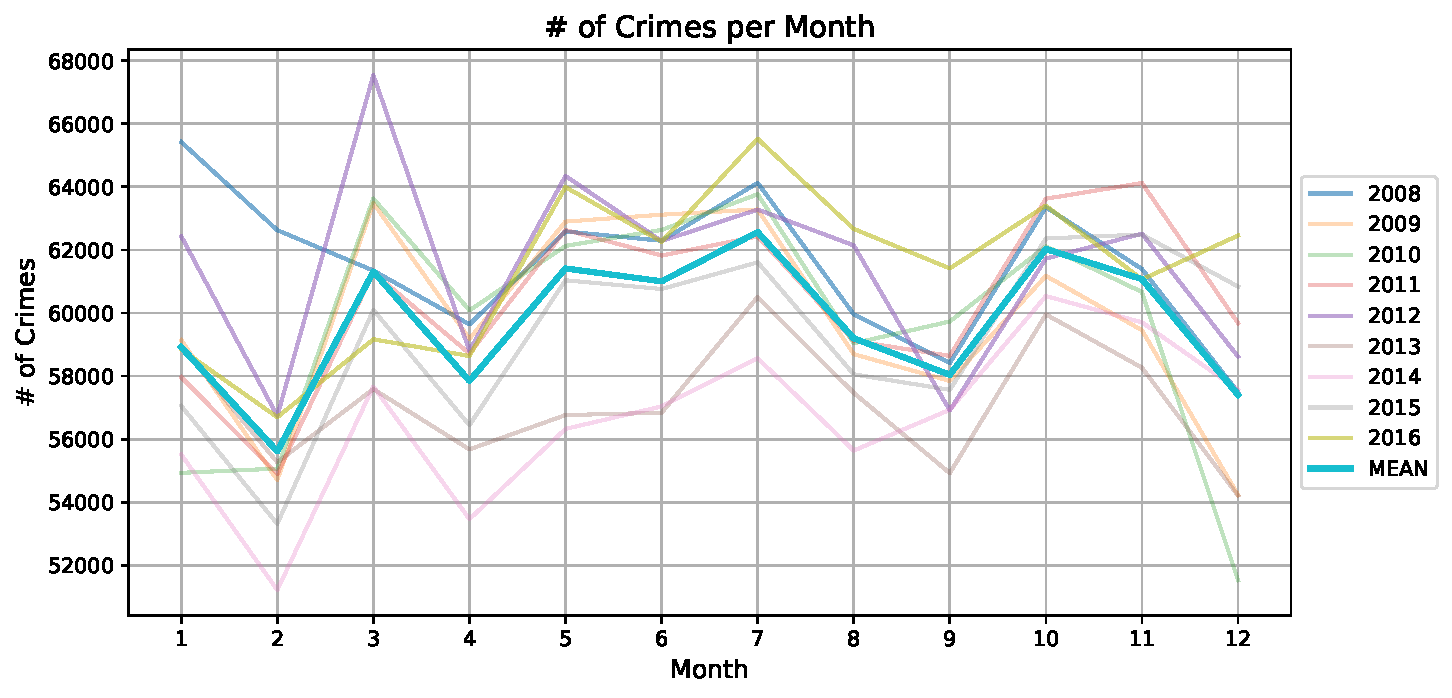
\includegraphics{../imgs/data_understanding/crimes_per_month.pdf}
                }
                \caption{Crime's progress over the months}
            \end{figure}
        \end{frame}

        \begin{frame}{Most Dangerous Years}
            \begin{figure}
                \centering
                \resizebox{\textwidth}{!}{
                    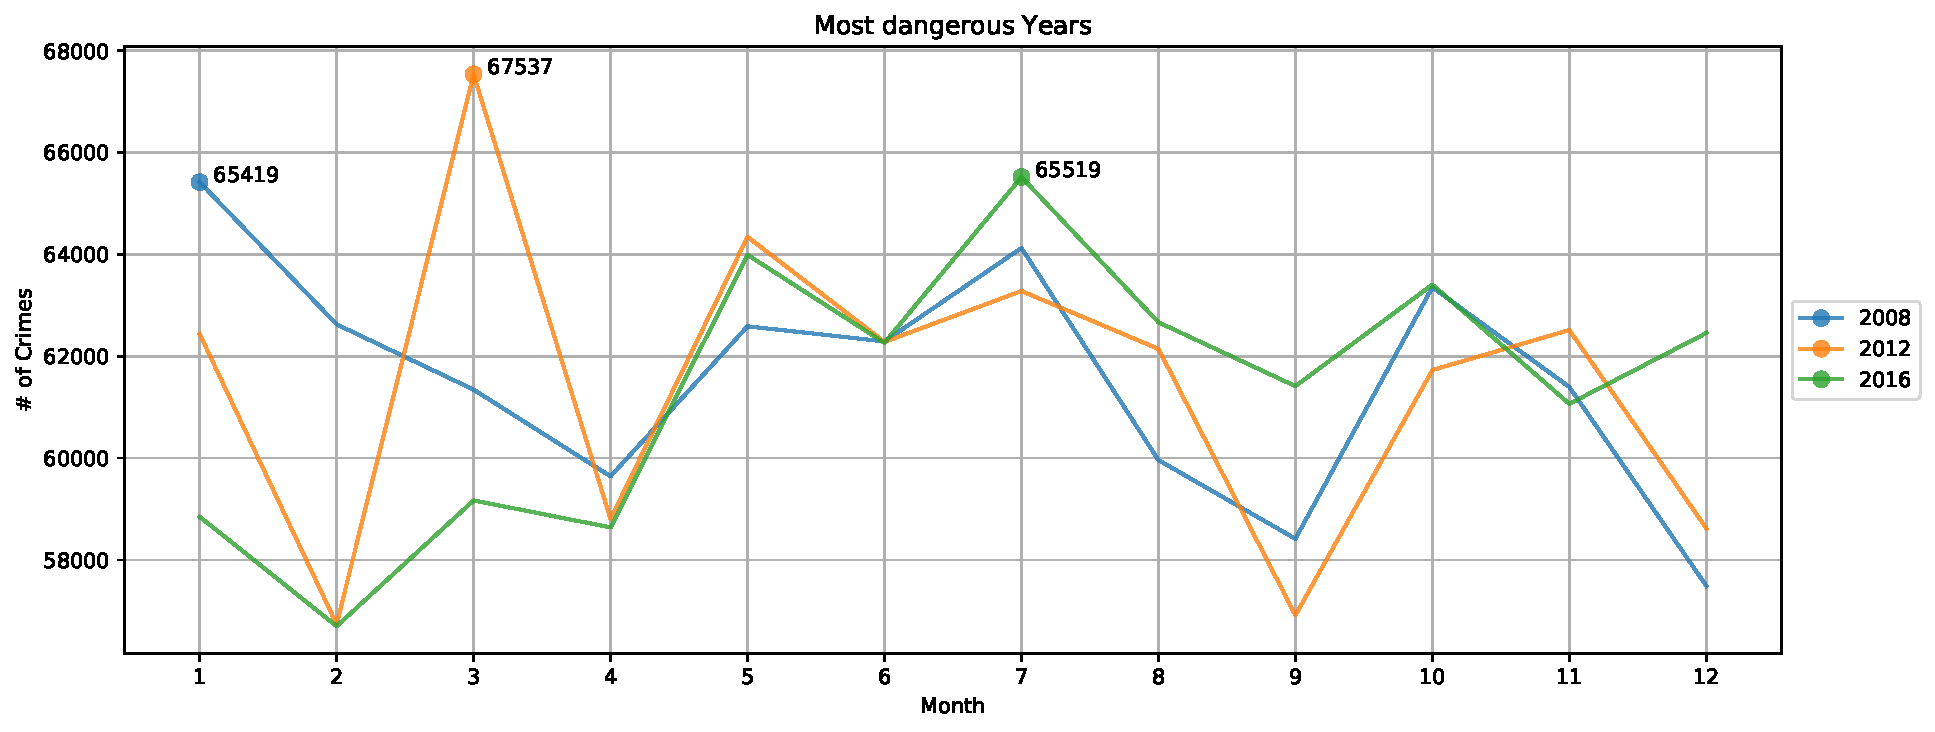
\includegraphics{../imgs/data_understanding/most_dangerous_years.pdf}
                }
            \end{figure}
        \end{frame}
    % section data_understanding (end)
\end{document}
